%----------------------------------------------------------------------------
%bb defines the bounding box for the pdf
%viewport defines the area of the pdf used
%in sidewaysfigure the last entry in bb moves the caption toward/away the pic
%in sidewaysfigure the second entry in bb moves the pic toward/away the caption
%----------------------------------------------------------------------------
\begin{figure}
\scalebox{0.8}[0.8]{
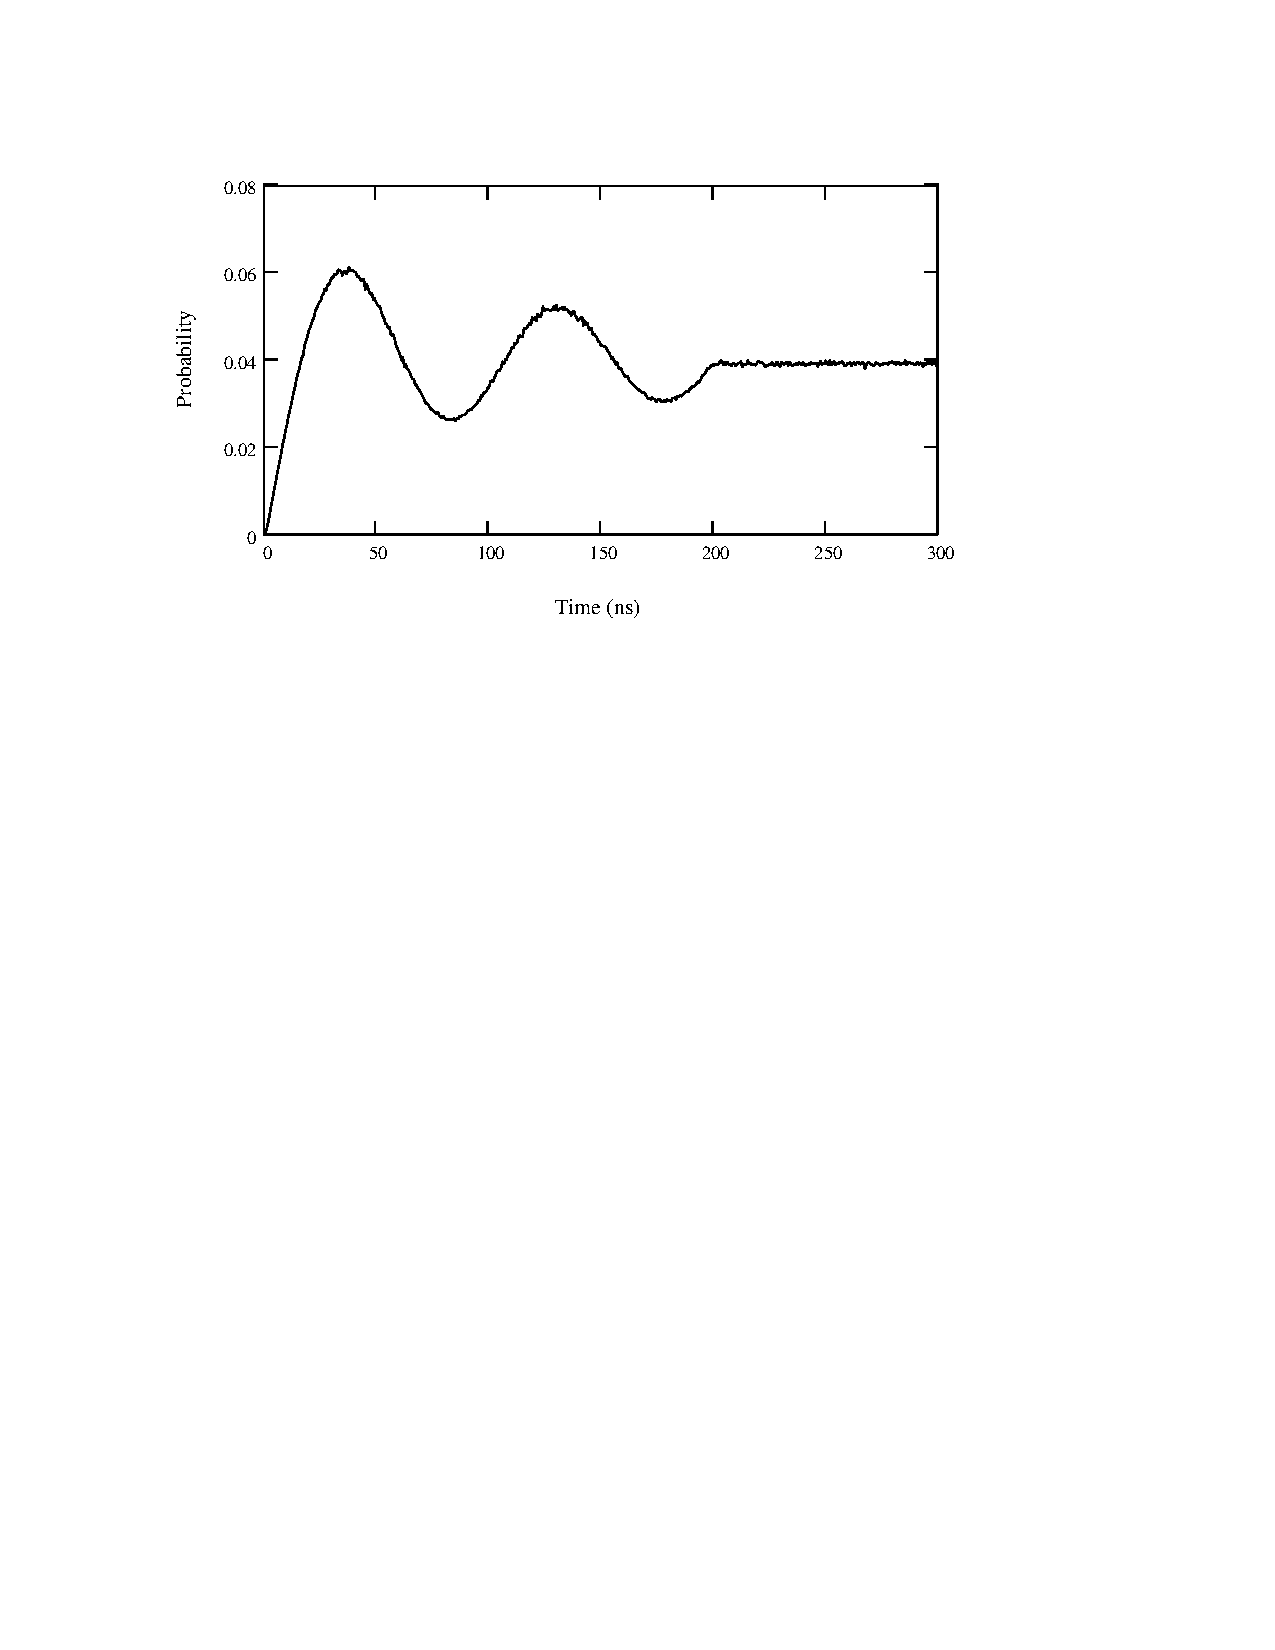
\includegraphics[bb=10 490 550 690]
{thermal_200/thermal_200.pdf}
}
\caption[Simulated thermal (Doppler and geometric) effects on observed fluorescence -- 200 ns pulse]{Simulated thermal (Doppler and geometric) effects on observed fluorescence -- 200 ns pulse. The calculations presented here have nearly the same parameters as Figure \ref{thermal_2} (left is ideal, right is polarization averaged) except these require a smaller fluence of 10 J/m$^2$ to induce two complete oscillations in 200 ns (instead of 1000 J/m$^2$ for 2 ns). The peak power of the pulse is 50 W -- four orders of magnitude larger than the typical CW HeNe laser.}
\label{thermal_200}
\end{figure}
%----------------------------------------------------------------------------
